\documentclass[10pt,aspectratio=169]{beamer}
\usepackage{graphicx}
\usepackage{booktabs,multirow,tabu}
\usepackage{tikz}
\usepackage{siunitx}
\usepackage[absolute,overlay]{textpos}
\usepackage{adjustbox}
\usepackage{feynmp}
\usepackage{tikz-feynman}
\tikzfeynmanset{compat=1.1.0}
\usepackage{bibentry}
\usepackage[style=verbose,backend=bibtex]{biblatex}

\nobibliography{weekly.bib}
%%%%%%%%%%%%%%%%%%%%%%%%%%%%%%

\usepackage{palatino}             % font
\setbeamercovered{transparent}    % uncover
\usetheme{metropolis}
\usefonttheme{serif}
\hypersetup{
  colorlinks = true,
}
\setbeamertemplate{footline}[frame number]
\setbeamertemplate{navigation symbols}{}
\setbeamerfont{author}{size=\large,series=\bfseries}
\setbeamerfont{date}{size=\normalsize}
\setbeamerfont{institute}{size=\normalsize}
\setbeamerfont{conference}{size=\normalsize,series=\bfseries}
\renewcommand{\instlogoA}{atlas}
\renewcommand{\instlogoB}{sydney}
\graphicspath{{logos/}{figures/}}

%%%%%%%%%%%%%%%%%%%%%%%%%%%%%%

\title{Sydney group update}
\author[]{Sydney group}
\date{\today}
\conference{Australian ATLAS Meeting}

\begin{document}
\begin{frame}\titlepage\end{frame}

%%%%%%%%%%%%%%%%%%%%%%%%%%%%%%%%%%%%%%%%%%%%%%%%%%%%%%%%%%%%%%%

\begin{frame}{Introduction: Four Tops Analysis}
  \begin{figure}
    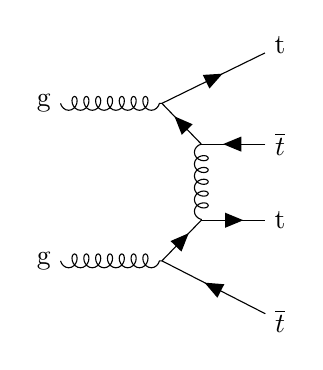
\begin{tikzpicture}
      \begin{feynman}
        % Define the gluons
        \vertex (g1s) {g}; 
        \vertex[right=1.5cm of g1s](g1e);
        
        \vertex[below=2.0cm of g1s](g2s){g};
        \vertex[right=1.5cm of g2s](g2e);

        %Draw all the tops in a line 
        \vertex[right=1.5cm of g1e](tmp); 
        \vertex[above=0.5cm of tmp](t1e) {t}; 
        \vertex[below=0.25cm of tmp](t2e) {\(\overline t\)}; 
        \vertex[below=1.25cm of tmp](t3e) {t}; 
        \vertex[below=2.5cm of tmp](t4e) {\(\overline t\)};
        
        %Draw start of tops 
        \vertex[left=1.0cm of t2e](t2s); 
        \vertex[left=1.0cm of t3e](t3s); 

        \diagram* {
          {[edges=gluon]
            (g1s) -- (g1e), 
            (g2s) -- (g2e), 
            (t2s) -- (t3s),
          }, 
          {[edges=fermion]
            (t2e) -- (t2s) -- (g1e) -- (t1e), 
            (t4e) -- (g2e) -- (t3s) -- (t3e),           
          },
        };
      \end{feynman}
    \end{tikzpicture}
    \bigskip
    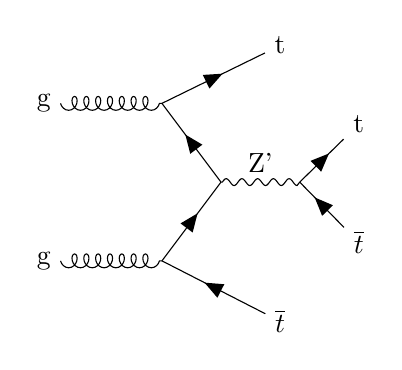
\begin{tikzpicture}
      \begin{feynman}
        % Define the gluons
        \vertex (g1s) {g}; 
        \vertex[right=1.5cm of g1s](g1e);
        
        \vertex[below=2.0cm of g1s](g2s){g};
        \vertex[right=1.5cm of g2s](g2e);

        %Draw all the tops in a line 
        \vertex[right=1.5cm of g1e](tmp); 
        \vertex[above=0.5cm of tmp](t1e) {t}; 
        \vertex[below=2.5cm of tmp](t4e) {\(\overline t\)};         
        
        % Resonance
        \vertex[below=1.0cm of tmp](tmp2); 
        \vertex[left=0.75cm of tmp2](Zs);
        \vertex[right=1.0cm of Zs](Ze); 
        \vertex[right=0.75cm of Ze](tmp3); 

        %Draw start of tops 
        \vertex[above=0.5cm of tmp3](t2e) {t};                   
        \vertex[below=0.5cm of tmp3](t3e) {\(\overline t\)};     

        \diagram* {
          {[edges=gluon]
            (g1s) -- (g1e), 
            (g2s) -- (g2e), 
          }, 
          {[edges=fermion]
            (g1e) -- (t1e), 
            (Zs) -- (g1e), 
            (g2e) -- (Zs),
            (t4e) -- (g2e), 
            (Ze) -- (t2e), 
            (t3e) -- (Ze),
          },
          {[edges=boson]
            (Zs) -- [edge label=Z'](Ze),
          },
        };
      \end{feynman}
    \end{tikzpicture}
    \caption{$t \bar{t} t \bar{t}$ production Feynman diagrams for left) Standard Model right) BSM Top-Philic model}
    \label{fig:Tops}
  \end{figure}
  \begin{itemize}
    \item Within the SM, the 4-top production is extremely rare ($\sigma = 12.6^{+5.6}_{-5.2}$fb) and occurs via gluon fusion.
    \item Some BSM physics models predict a boosting of this cross-section from modified top quark couplings or heavy resonances (Figure \ref{fig:Tops}).  
  \end{itemize}
\end{frame}

\begin{frame}{Introduction: Four Tops Analysis}
  \begin{itemize}
    \item Products of resonance tops are expected to be largely boosted and produce fat-jets. 
    \item These jet types can be reclustered into so called RC-jets in single lepton analyses.
    \item Graph Neural Networks (GNNs) could potentially assist in identifying jets originating from resonance tops.
    \item Although the data science technique has been around since 2009, it only recently gained mainstream and HEPP attention. 
    \item A similar problem was partially solved using GNNs to group jets to common parents in the $ttH$ production at Berkeley.
  \end{itemize}
\end{frame}

\begin{frame}{What is a Graph Neural Network?}
  \begin{figure} 
    \includegraphics[scale=0.2]{Graph}
  \end{figure}

  \begin{itemize}
    \item A Graph Neural Network is a generalized deep learning technique similar to a conventional Neural Network (Deep Layers, Aggregation, Convolution, Pooling etc.)
    \item What makes a GNN unique is that, non-euclidean sampled data can be encoded on graph data structures where in the context of HEPP; 
    \begin{itemize}
      \item Nodes - Some object (Particle, Jets) that has attributes ($\eta$, $\phi$, $p_T$, ...)
      \item Edges - Some relation between objects; $\Delta$R, Inv Mass, $\Delta$(*).  
      \item Graph - Some global properties of the graph; Collision Energy, Missing $p_T$, $\phi$...  
    \end{itemize}  
  \end{itemize}
\end{frame}

\begin{frame}{What is a Graph Neural Network?}
  \begin{figure} 
    \begin{tikzpicture}
      \node[anchor=north west, inner sep=0](image) at (0,0)
      {\includegraphics[scale=0.2]{Graph}};
      \begin{scope}[x={(image.south east)},y={(image.south west)}]
        \draw[red,ultra thick,rounded corners](0.0, 0.1) rectangle (0.35,0.7);
      \end{scope}
    \end{tikzpicture}
  \end{figure}

  Given some graph data structure, with edge and node features, an example computation would look something like this:
  \begin{itemize}
    \item Trainable edge weights are first updated via a multilayer-perceptron (MLP).
    \item The inputs of the MLP are the current edge state, attributes from \textit{sender} and \textit{receiver} nodes, and some global value.
    \item Edges are finally updated through a permutation invariant function; summation, averaging, max, min, ... 
    \item This allows for edges to be mapped appropriately to nodes.
  \end{itemize}
\end{frame}

\begin{frame}{What is a Graph Neural Network?}
  \begin{figure} 
    \begin{tikzpicture}
      \node[anchor=north west, inner sep=0](image) at (0.35,0)
      {\includegraphics[scale=0.2]{Graph}};
      \begin{scope}[x={(image.south east)},y={(image.south west)}]
        \draw[red,ultra thick,rounded corners](0.38,-0.25) rectangle (0.68,0.35);
      \end{scope}
    \end{tikzpicture}
  \end{figure}
  
  \begin{itemize}
    \item Nodes are updated by applying an MLP to the node features and updated incoming edge attributes. 
    \item Using the updated edges and nodes of the graph, a permutation invariant function is again used to map to a global value or attribute.
  \end{itemize}
\end{frame}


\begin{frame}{What is a Graph Neural Network?}
  \begin{figure} 
    \begin{tikzpicture}
      \node[anchor=north west, inner sep=0](image) at (0.0,0)
      {\includegraphics[scale=0.2]{Graph}};
      \begin{scope}[x={(image.south east)},y={(image.south west)}]
        \draw[red,ultra thick,rounded corners](0.68,-0.6) rectangle (1,0.1);
      \end{scope}
    \end{tikzpicture}
  \end{figure}
  
  \begin{itemize}
    \item Finally, a global attribute update is performed with the global attribute value and updated edge and node vectors.
    \item The described sequence is \textbf{not} necessarily enforced, but can be adjusted arbitrarily, adding to the flexibility of GNNs.
    \item This flexibility has opened many new architectures; Auto-encoding, Node/Edge predictions, Graph Convolution Neural Networks, Multi-Block models, ...
  \end{itemize}
\end{frame}

\begin{frame}{My Current Progress in Implementing GNNs}
  \begin{itemize}
    \item I have been writing most of the infrastructure code;
    \begin{itemize}
      \item Reading multiple ROOT files (containing resonance events)
      \item Converting particle objects; jets, electrons, muons, truth particles, tops, ... into python objects for matching 
      \item Matching truth particles to truth jets and matching truth jets to detector jets using a $\Delta$R matching technique.
      \item Integrated a very basic working GNN into the code using pytorch-geometric.
    \end{itemize}
    \item But there are still some issues that need resolving:
    \begin{itemize}
      \item Truth jet and truth particle matching using $\Delta$R is not very unreliable (likely due to gluons and any quarks below charm given a flavor value of 0).
      \item Jet and truth jet matching is also experiencing the same issue.
    \end{itemize}
    \item Next things to work on:
    \begin{itemize}
      \item Exploring more GNN architectures and comparing their performance on the truth children (perfectly matching tops).
      \item Understanding how to properly match jets and truth jets to truth children.
    \end{itemize}
  \end{itemize}
\end{frame}

\begin{frame}{My Current Progress in Implementing GNNs}
  \begin{figure} 
    \includegraphics[scale=0.22]{Weird}
  \end{figure}
\end{frame}

\begin{frame}{Fin}
  \begin{center}
    \textbf{Thanks for Listening!}
  \end{center}
  \fullcite{Inductive}
  \fullcite{Sirunyan_2020}
  \fullcite{Kim_2016}
\end{frame}






%%%%%%%%%%%%%%%%%%%%%%%%%%%%%%%%%%%%%%%%%%%%%%%%%%%%%%%%%%%%%%%

\end{document}
